\documentclass[a4paper,12pt]{article}

\usepackage{rotating}
\usepackage[top=1in, bottom=1in, left=0.75in, right=0.75in]{geometry}
\usepackage{graphicx}
\usepackage[numbers,square,sort&compress]{natbib}
\usepackage{setspace}
\usepackage[cdot,mediumqspace,]{SIunits}
\usepackage{caption}
\usepackage{subcaption}
\usepackage{mathtools}
\usepackage{authblk}
\usepackage{float}
\renewcommand{\thesubsection}{\thesection.\alph{subsection}}
\providecommand{\e}[1]{\ensuremath{\times 10^{#1}}}

\begin{document}
\onehalfspacing
\title{PHY 407 Lab 6}
\author{Natalie Price-Jones, 999091021}
\date{17 October 2014}
\affil{\small{natalie.price.jones@mail.utoronto.ca}}
\maketitle

\section{Question 1}

\begin{figure}[H]
\centering
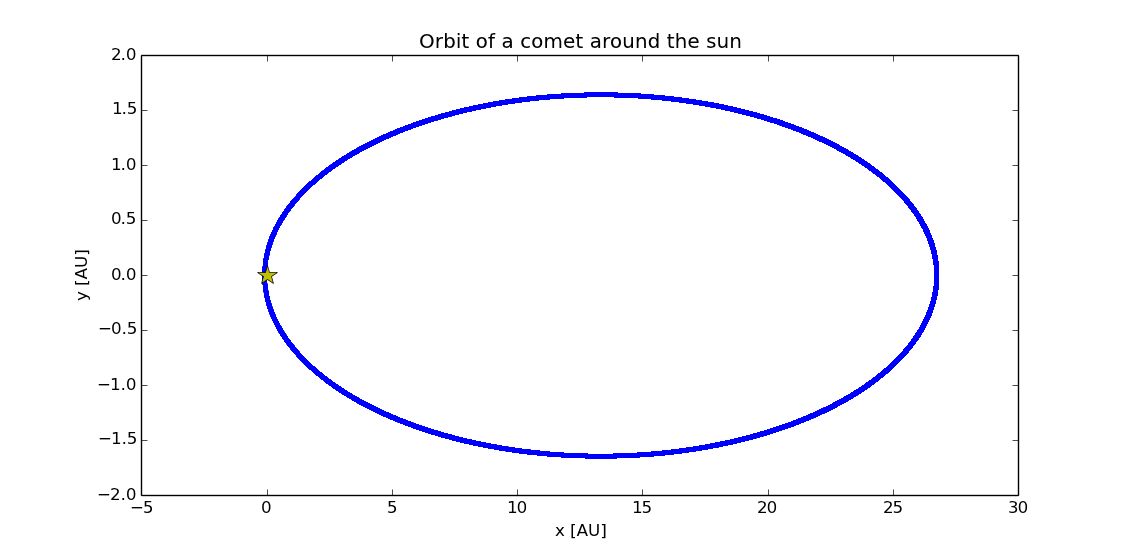
\includegraphics[width = \linewidth]{lab6q1.png}
\caption{}
\label{fig:q1}
\end{figure}
 
Figure \ref{fig:q1} was made with a step size of 0.0005 years. The calculation took, on average, about 42 seconds to run.

\section{Question 2}

\begin{figure}[H]
\centering
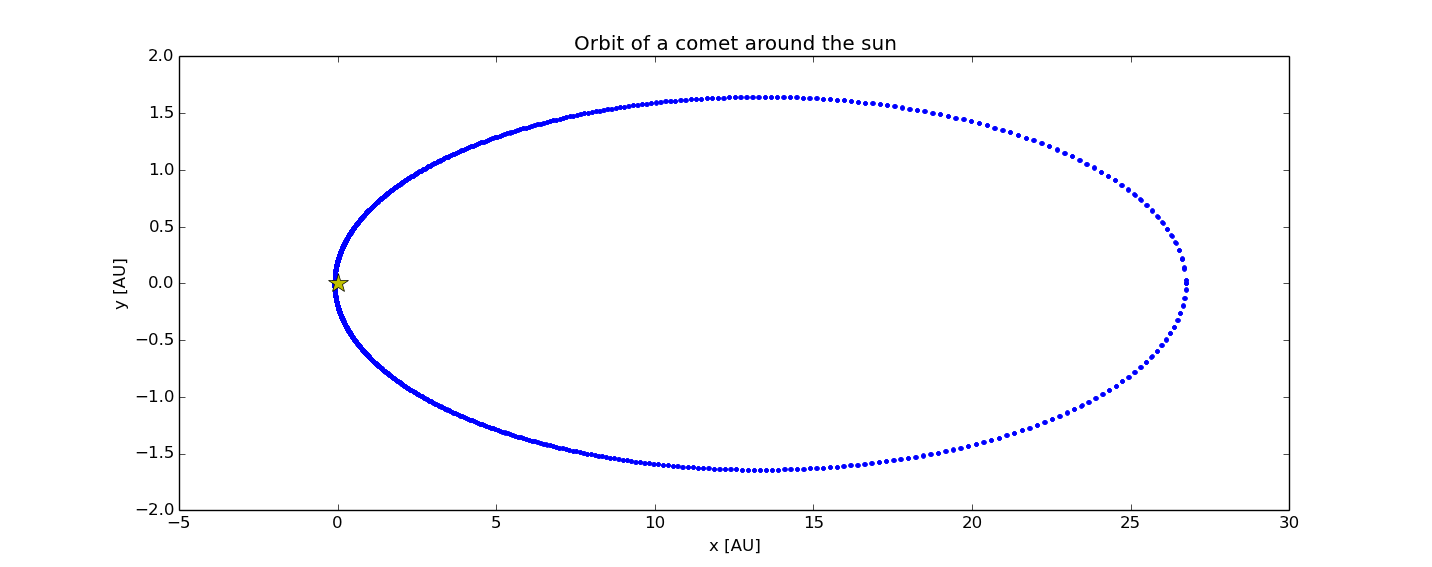
\includegraphics[width = \linewidth]{lab6q2.png}
\caption{}
\label{fig:q2}
\end{figure}

Figure \ref{fig:q2} was made with varying step size, shown in Figure \ref{fig:q2i}. The calculation took, on average, 0.65 seconds to run. This is a vast improvement on the fixed step size method. The trade off came in the error, which on average was $3.8\e{-10} AU$, compared with $2.5\e{-12} AU$ in the previous part. This error could be adjusted, however, by chaning the $\delta$ parameter that determined the desired level of accuracy. If $\delta$ was changed from 1 km to 1 m, for exmaple, runtime increased to about 5 seconds, but error was reduced to $6.0\e{-14} AU$.

\begin{figure}[H]
\centering
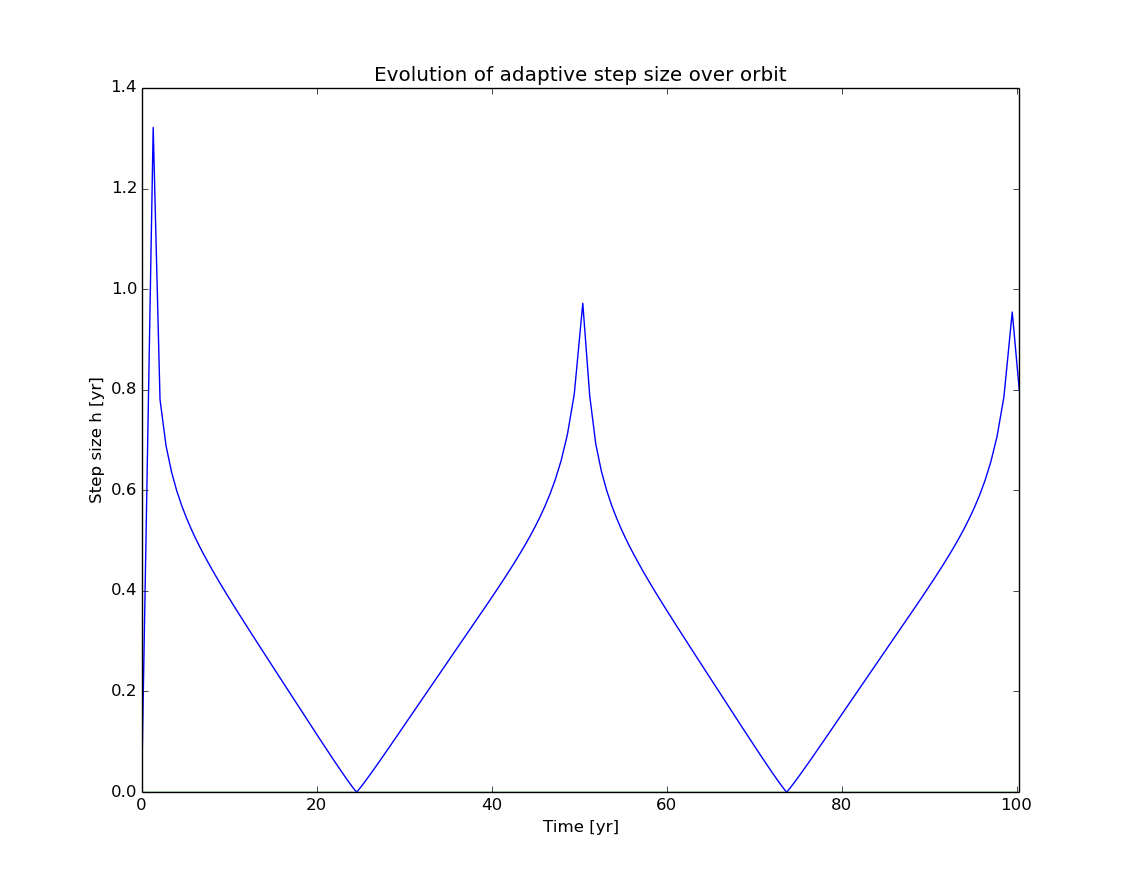
\includegraphics[width = \linewidth]{lab6q2additional.png}
\caption{}
\label{fig:q2i}
\end{figure}

\section{Question 3}

\begin{figure}[H]
\centering
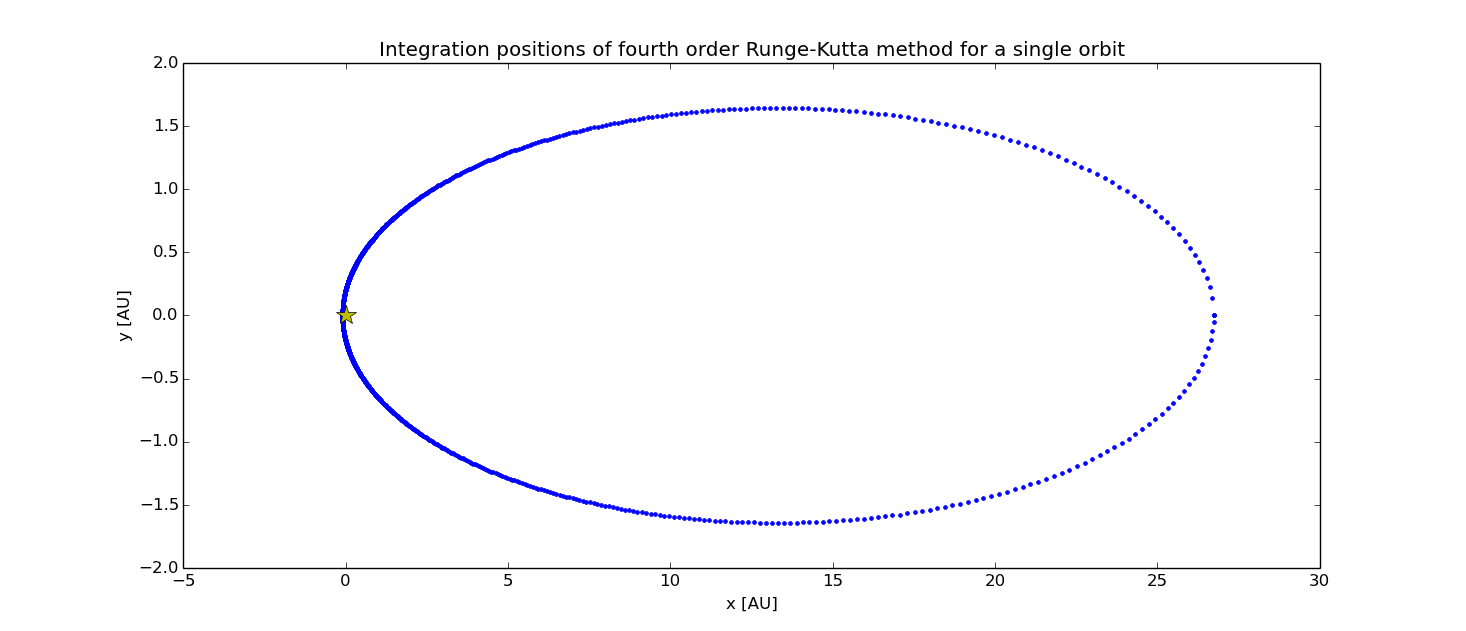
\includegraphics[width = \linewidth]{lab6q3.png}
\caption{}
\label{fig:q3}
\end{figure}

\section{Question 5}

\subsection{Part a)}
\begin{figure}[H]
\centering
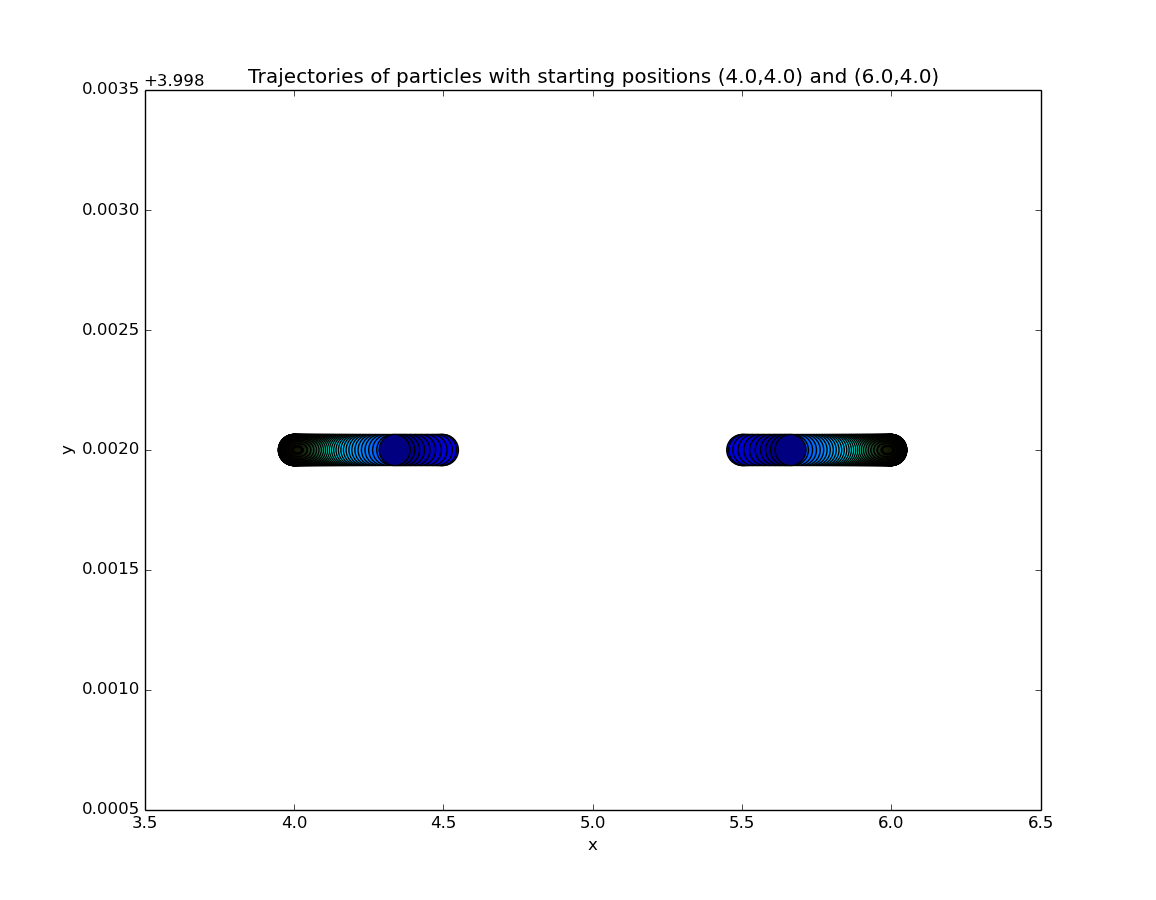
\includegraphics[width = \linewidth]{lab6q5a.png}
\caption{}
\label{fig:q5a}
\end{figure}

\begin{figure}[H]
\centering
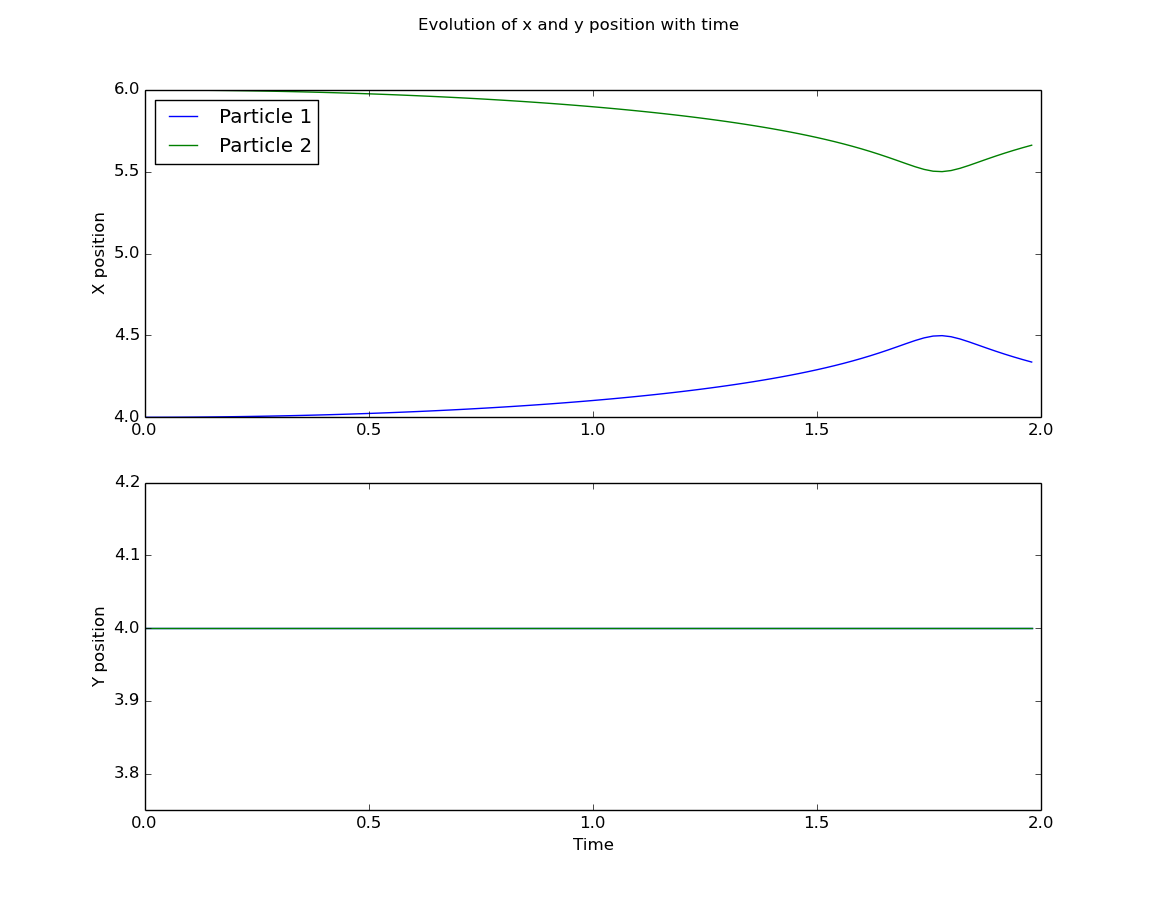
\includegraphics[width = \linewidth]{lab6q5ai.png}
\caption{}
\label{fig:q5ai}
\end{figure}

\subsection{Part b)}

\begin{figure}[H]
\centering
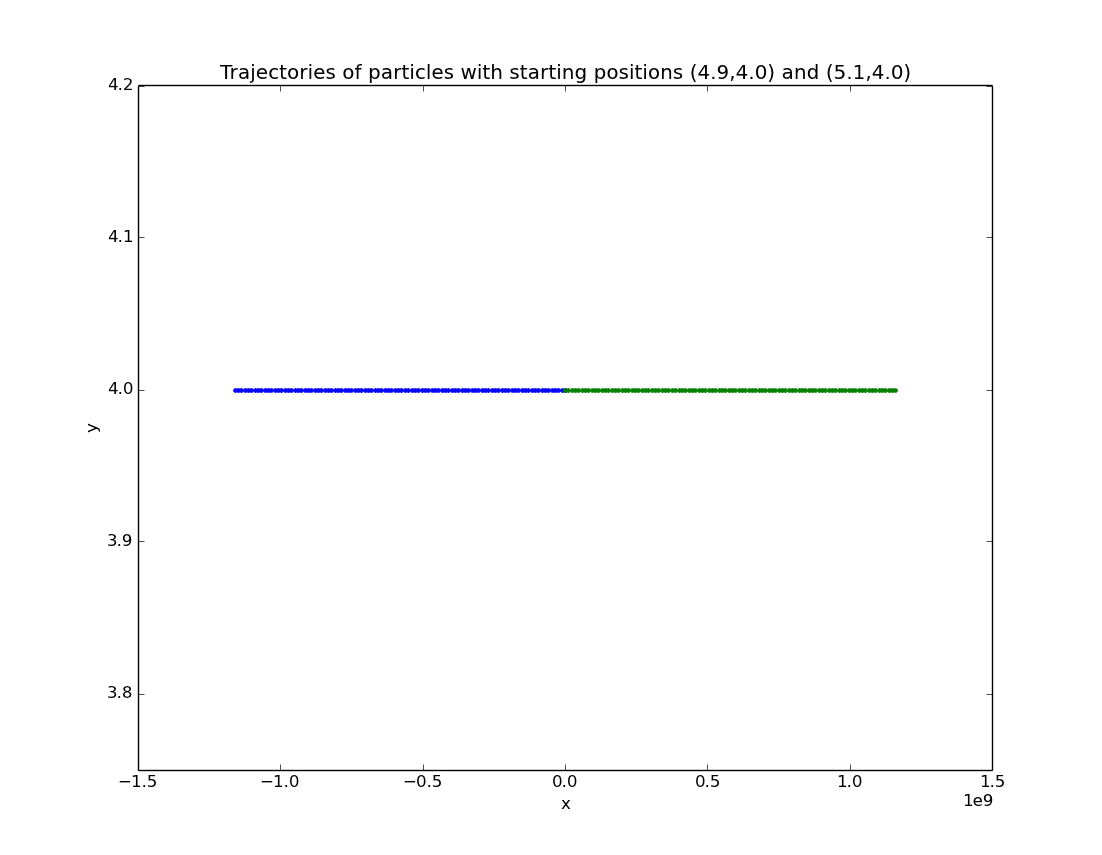
\includegraphics[width = \linewidth]{lab6q5b.png}
\caption{}
\label{fig:q5b}
\end{figure}

\begin{figure}[H]
\centering
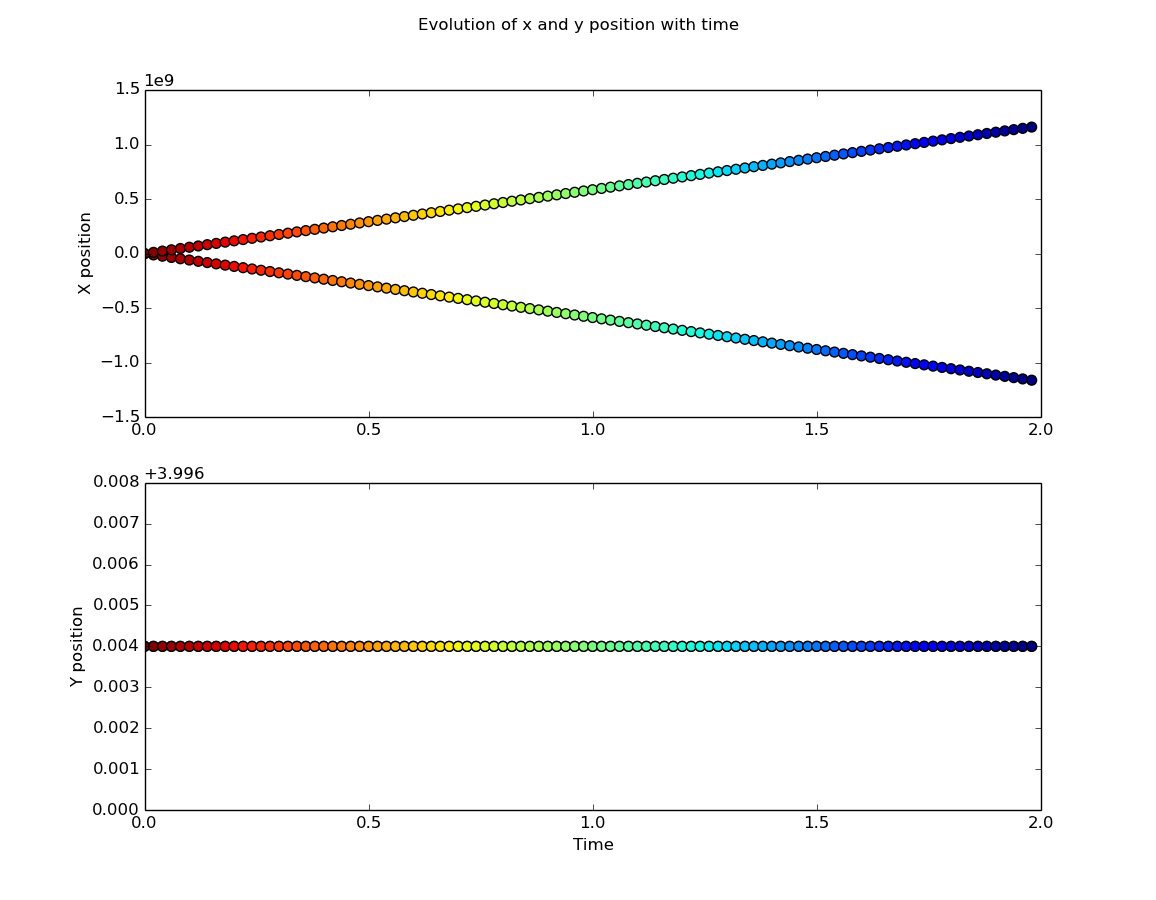
\includegraphics[width = \linewidth]{lab6q5bi.png}
\caption{}
\label{fig:q5bi}
\end{figure}

\subsection{Part c)}

\begin{figure}[H]
\centering
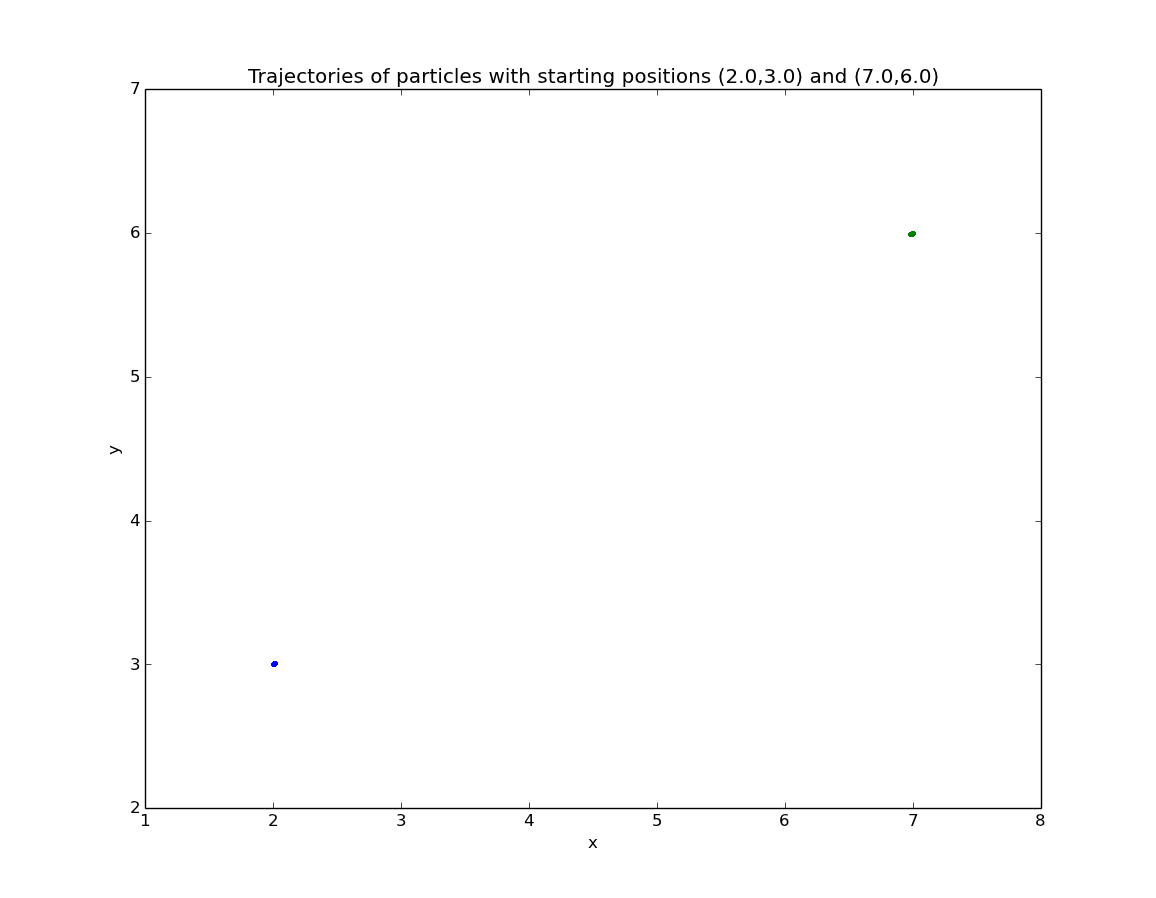
\includegraphics[width = \linewidth]{lab6q5c.png}
\caption{}
\label{fig:q5c}
\end{figure}

\begin{figure}[H]
\centering
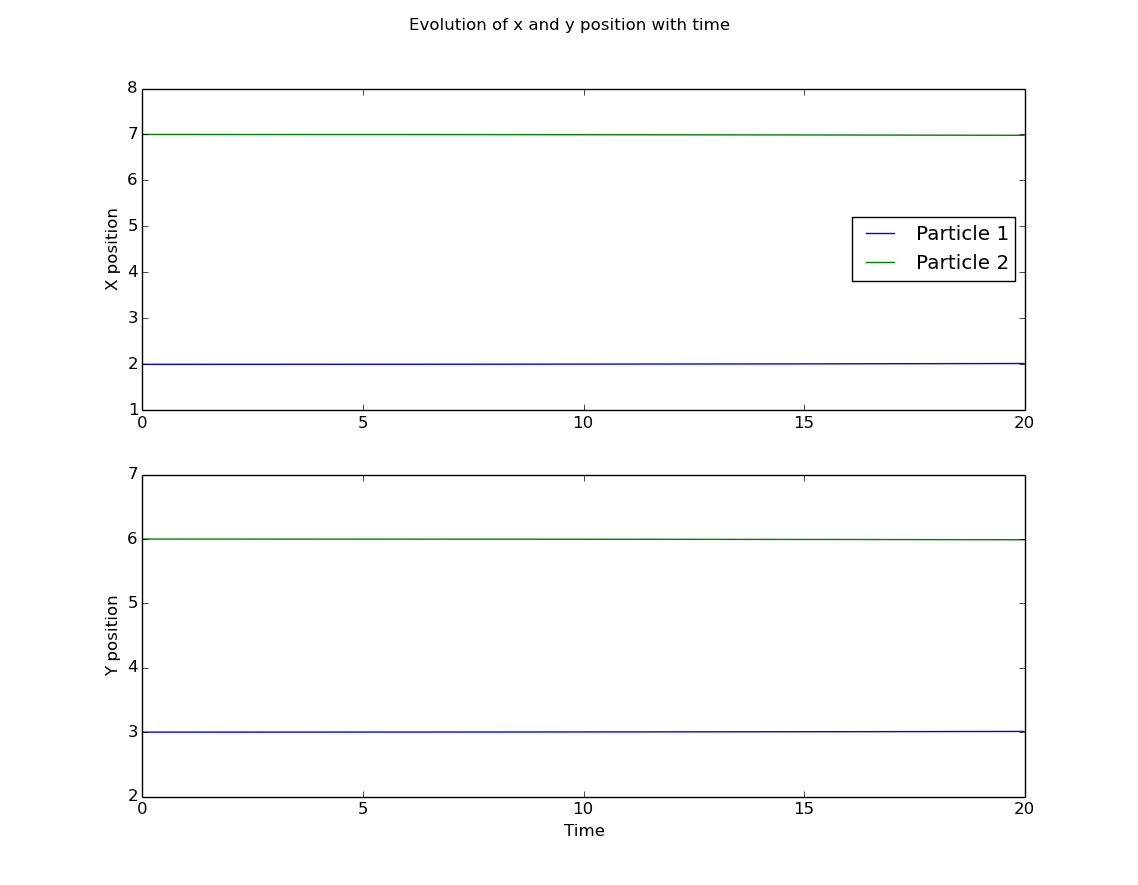
\includegraphics[width = \linewidth]{lab6q5ci.png}
\caption{}
\label{fig:q5ci}
\end{figure}

\section{Question 6}

\begin{figure}[H]
\centering
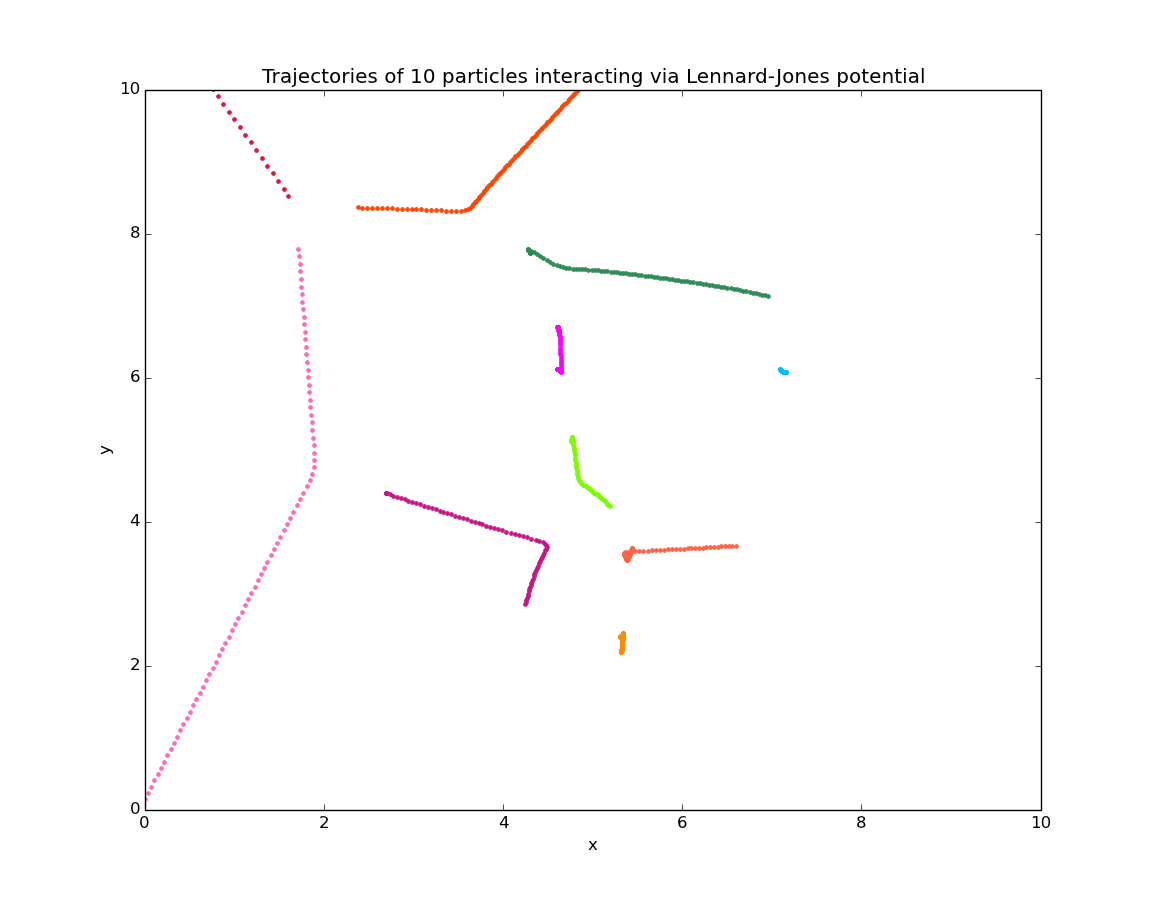
\includegraphics[width = \linewidth]{lab6q6_1.png}
\caption{}
\label{fig:q6}
\end{figure}

\section{Question 7}

\begin{figure}[H]
\centering
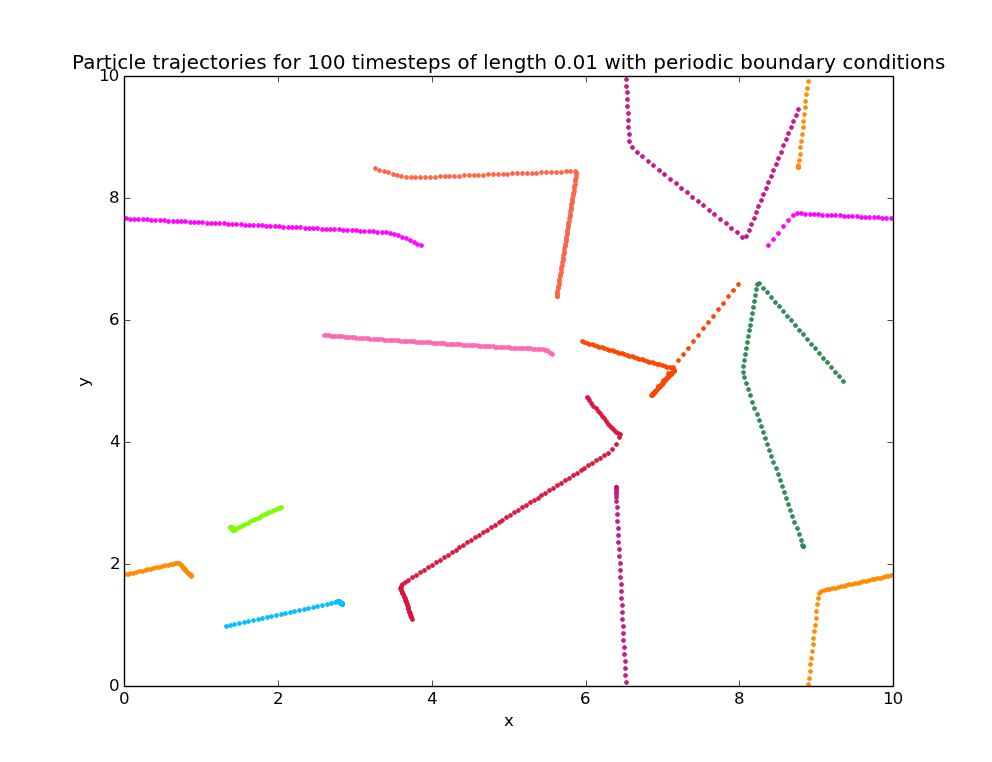
\includegraphics[width = \linewidth]{lab6q7.png}
\caption{}
\label{fig:q7}
\end{figure}

\begin{figure}[H]
\centering
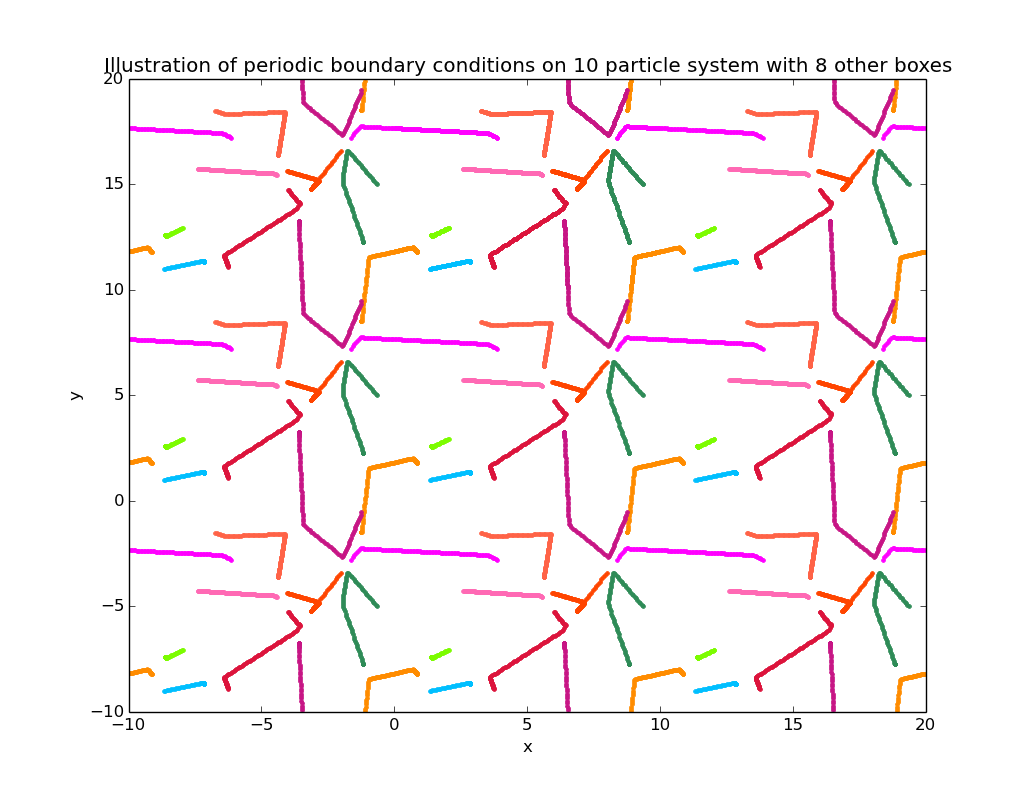
\includegraphics[width = \linewidth]{lab6q7additional.png}
\caption{}
\label{fig:q7i}
\end{figure}

\section{Question 8}

\begin{figure}[H]
\centering
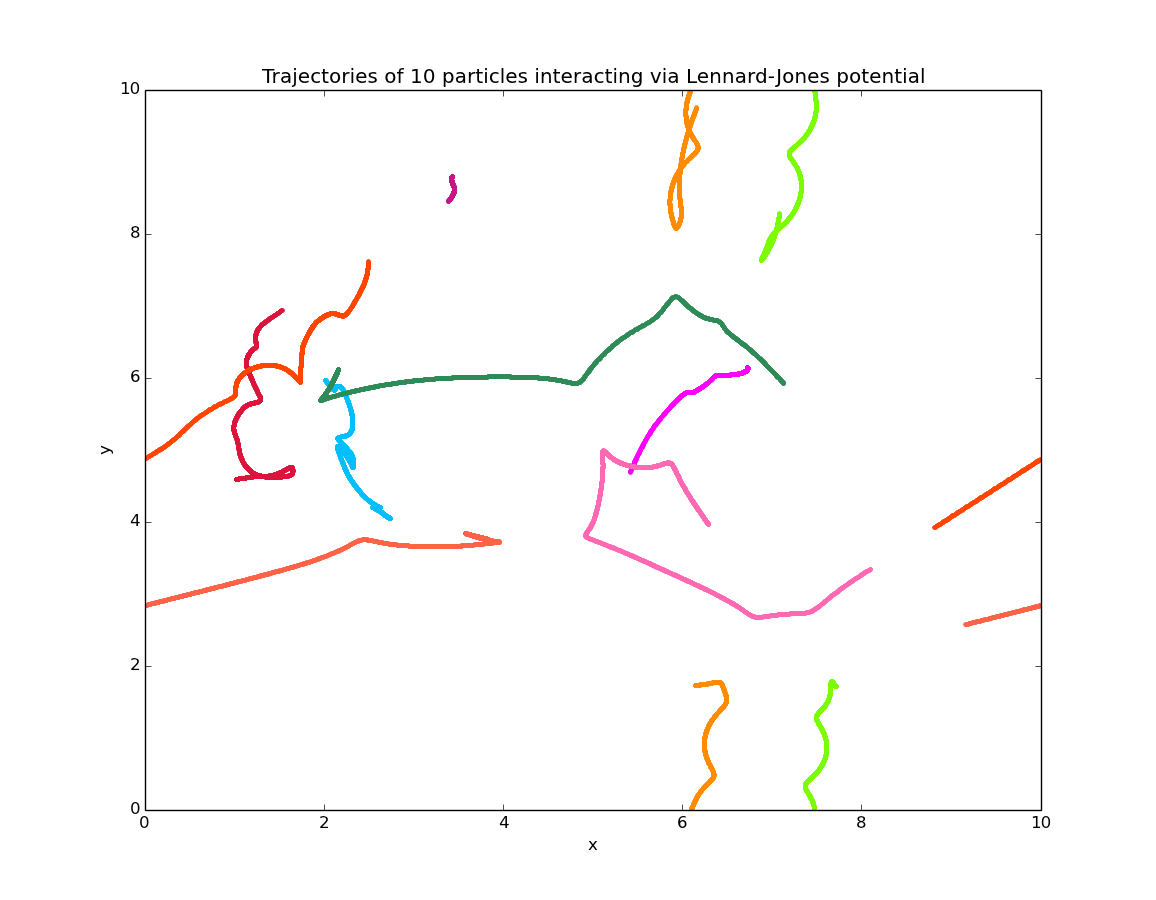
\includegraphics[width = \linewidth]{lab6q8.png}
\caption{}
\label{fig:q8}
\end{figure}

\end{document}





